% Options for packages loaded elsewhere
\PassOptionsToPackage{unicode}{hyperref}
\PassOptionsToPackage{hyphens}{url}
%
\documentclass[
]{article}
\usepackage{amsmath,amssymb}
\usepackage{iftex}
\ifPDFTeX
  \usepackage[T1]{fontenc}
  \usepackage[utf8]{inputenc}
  \usepackage{textcomp} % provide euro and other symbols
\else % if luatex or xetex
  \usepackage{unicode-math} % this also loads fontspec
  \defaultfontfeatures{Scale=MatchLowercase}
  \defaultfontfeatures[\rmfamily]{Ligatures=TeX,Scale=1}
\fi
\usepackage{lmodern}
\ifPDFTeX\else
  % xetex/luatex font selection
\fi
% Use upquote if available, for straight quotes in verbatim environments
\IfFileExists{upquote.sty}{\usepackage{upquote}}{}
\IfFileExists{microtype.sty}{% use microtype if available
  \usepackage[]{microtype}
  \UseMicrotypeSet[protrusion]{basicmath} % disable protrusion for tt fonts
}{}
\makeatletter
\@ifundefined{KOMAClassName}{% if non-KOMA class
  \IfFileExists{parskip.sty}{%
    \usepackage{parskip}
  }{% else
    \setlength{\parindent}{0pt}
    \setlength{\parskip}{6pt plus 2pt minus 1pt}}
}{% if KOMA class
  \KOMAoptions{parskip=half}}
\makeatother
\usepackage{xcolor}
\usepackage[margin=1in]{geometry}
\usepackage{color}
\usepackage{fancyvrb}
\newcommand{\VerbBar}{|}
\newcommand{\VERB}{\Verb[commandchars=\\\{\}]}
\DefineVerbatimEnvironment{Highlighting}{Verbatim}{commandchars=\\\{\}}
% Add ',fontsize=\small' for more characters per line
\usepackage{framed}
\definecolor{shadecolor}{RGB}{248,248,248}
\newenvironment{Shaded}{\begin{snugshade}}{\end{snugshade}}
\newcommand{\AlertTok}[1]{\textcolor[rgb]{0.94,0.16,0.16}{#1}}
\newcommand{\AnnotationTok}[1]{\textcolor[rgb]{0.56,0.35,0.01}{\textbf{\textit{#1}}}}
\newcommand{\AttributeTok}[1]{\textcolor[rgb]{0.13,0.29,0.53}{#1}}
\newcommand{\BaseNTok}[1]{\textcolor[rgb]{0.00,0.00,0.81}{#1}}
\newcommand{\BuiltInTok}[1]{#1}
\newcommand{\CharTok}[1]{\textcolor[rgb]{0.31,0.60,0.02}{#1}}
\newcommand{\CommentTok}[1]{\textcolor[rgb]{0.56,0.35,0.01}{\textit{#1}}}
\newcommand{\CommentVarTok}[1]{\textcolor[rgb]{0.56,0.35,0.01}{\textbf{\textit{#1}}}}
\newcommand{\ConstantTok}[1]{\textcolor[rgb]{0.56,0.35,0.01}{#1}}
\newcommand{\ControlFlowTok}[1]{\textcolor[rgb]{0.13,0.29,0.53}{\textbf{#1}}}
\newcommand{\DataTypeTok}[1]{\textcolor[rgb]{0.13,0.29,0.53}{#1}}
\newcommand{\DecValTok}[1]{\textcolor[rgb]{0.00,0.00,0.81}{#1}}
\newcommand{\DocumentationTok}[1]{\textcolor[rgb]{0.56,0.35,0.01}{\textbf{\textit{#1}}}}
\newcommand{\ErrorTok}[1]{\textcolor[rgb]{0.64,0.00,0.00}{\textbf{#1}}}
\newcommand{\ExtensionTok}[1]{#1}
\newcommand{\FloatTok}[1]{\textcolor[rgb]{0.00,0.00,0.81}{#1}}
\newcommand{\FunctionTok}[1]{\textcolor[rgb]{0.13,0.29,0.53}{\textbf{#1}}}
\newcommand{\ImportTok}[1]{#1}
\newcommand{\InformationTok}[1]{\textcolor[rgb]{0.56,0.35,0.01}{\textbf{\textit{#1}}}}
\newcommand{\KeywordTok}[1]{\textcolor[rgb]{0.13,0.29,0.53}{\textbf{#1}}}
\newcommand{\NormalTok}[1]{#1}
\newcommand{\OperatorTok}[1]{\textcolor[rgb]{0.81,0.36,0.00}{\textbf{#1}}}
\newcommand{\OtherTok}[1]{\textcolor[rgb]{0.56,0.35,0.01}{#1}}
\newcommand{\PreprocessorTok}[1]{\textcolor[rgb]{0.56,0.35,0.01}{\textit{#1}}}
\newcommand{\RegionMarkerTok}[1]{#1}
\newcommand{\SpecialCharTok}[1]{\textcolor[rgb]{0.81,0.36,0.00}{\textbf{#1}}}
\newcommand{\SpecialStringTok}[1]{\textcolor[rgb]{0.31,0.60,0.02}{#1}}
\newcommand{\StringTok}[1]{\textcolor[rgb]{0.31,0.60,0.02}{#1}}
\newcommand{\VariableTok}[1]{\textcolor[rgb]{0.00,0.00,0.00}{#1}}
\newcommand{\VerbatimStringTok}[1]{\textcolor[rgb]{0.31,0.60,0.02}{#1}}
\newcommand{\WarningTok}[1]{\textcolor[rgb]{0.56,0.35,0.01}{\textbf{\textit{#1}}}}
\usepackage{graphicx}
\makeatletter
\def\maxwidth{\ifdim\Gin@nat@width>\linewidth\linewidth\else\Gin@nat@width\fi}
\def\maxheight{\ifdim\Gin@nat@height>\textheight\textheight\else\Gin@nat@height\fi}
\makeatother
% Scale images if necessary, so that they will not overflow the page
% margins by default, and it is still possible to overwrite the defaults
% using explicit options in \includegraphics[width, height, ...]{}
\setkeys{Gin}{width=\maxwidth,height=\maxheight,keepaspectratio}
% Set default figure placement to htbp
\makeatletter
\def\fps@figure{htbp}
\makeatother
\setlength{\emergencystretch}{3em} % prevent overfull lines
\providecommand{\tightlist}{%
  \setlength{\itemsep}{0pt}\setlength{\parskip}{0pt}}
\setcounter{secnumdepth}{-\maxdimen} % remove section numbering
\ifLuaTeX
  \usepackage{selnolig}  % disable illegal ligatures
\fi
\usepackage{bookmark}
\IfFileExists{xurl.sty}{\usepackage{xurl}}{} % add URL line breaks if available
\urlstyle{same}
\hypersetup{
  pdftitle={Reproducible Research: Peer Assessment 1},
  hidelinks,
  pdfcreator={LaTeX via pandoc}}

\title{Reproducible Research: Peer Assessment 1}
\author{}
\date{\vspace{-2.5em}}

\begin{document}
\maketitle

\subsection{Loading and preprocessing the
data}\label{loading-and-preprocessing-the-data}

\begin{Shaded}
\begin{Highlighting}[]
\NormalTok{activity }\OtherTok{\textless{}{-}} \FunctionTok{read.csv}\NormalTok{(}\StringTok{"activity.csv"}\NormalTok{)}
\NormalTok{activity}\SpecialCharTok{$}\NormalTok{date }\OtherTok{\textless{}{-}} \FunctionTok{as.POSIXct}\NormalTok{(activity}\SpecialCharTok{$}\NormalTok{date)}
\FunctionTok{head}\NormalTok{(activity)}
\end{Highlighting}
\end{Shaded}

\begin{verbatim}
##   steps       date interval
## 1    NA 2012-10-01        0
## 2    NA 2012-10-01        5
## 3    NA 2012-10-01       10
## 4    NA 2012-10-01       15
## 5    NA 2012-10-01       20
## 6    NA 2012-10-01       25
\end{verbatim}

Let's see how big the dataset is:

\begin{Shaded}
\begin{Highlighting}[]
\FunctionTok{dim}\NormalTok{(activity)}
\end{Highlighting}
\end{Shaded}

\begin{verbatim}
## [1] 17568     3
\end{verbatim}

\subsection{What is mean total number of steps taken per
day?}\label{what-is-mean-total-number-of-steps-taken-per-day}

We will use \emph{tapply} funciton to calculate that:

\begin{Shaded}
\begin{Highlighting}[]
\NormalTok{tbl }\OtherTok{\textless{}{-}} \FunctionTok{tapply}\NormalTok{(activity}\SpecialCharTok{$}\NormalTok{steps, activity}\SpecialCharTok{$}\NormalTok{date, sum)}
\NormalTok{tbl }\OtherTok{\textless{}{-}} \FunctionTok{as.data.frame}\NormalTok{(tbl)}
\NormalTok{tbl}\SpecialCharTok{$}\NormalTok{date }\OtherTok{\textless{}{-}} \FunctionTok{as.POSIXct}\NormalTok{(}\FunctionTok{row.names}\NormalTok{(tbl))}

\FunctionTok{mean}\NormalTok{(tbl}\SpecialCharTok{$}\NormalTok{tbl, }\AttributeTok{na.rm=}\ConstantTok{TRUE}\NormalTok{)}
\end{Highlighting}
\end{Shaded}

\begin{verbatim}
## [1] 10766.19
\end{verbatim}

So the mean total number of steps taken per day equals \emph{10766.19}.

\subsection{What is median total number of steps taken per
day?}\label{what-is-median-total-number-of-steps-taken-per-day}

\begin{Shaded}
\begin{Highlighting}[]
\FunctionTok{median}\NormalTok{(tbl}\SpecialCharTok{$}\NormalTok{tbl, }\AttributeTok{na.rm=}\ConstantTok{TRUE}\NormalTok{)}
\end{Highlighting}
\end{Shaded}

\begin{verbatim}
## [1] 10765
\end{verbatim}

So the median total number of steps taken per day equals \emph{10765}.

Histogram of the total number of steps taken each day:

\begin{Shaded}
\begin{Highlighting}[]
\FunctionTok{hist}\NormalTok{(tbl}\SpecialCharTok{$}\NormalTok{tbl,}\AttributeTok{xlab=}\StringTok{"steps"}\NormalTok{, }\AttributeTok{main=}\StringTok{"Histogram of total number of steps taken per day"}\NormalTok{)}
\end{Highlighting}
\end{Shaded}

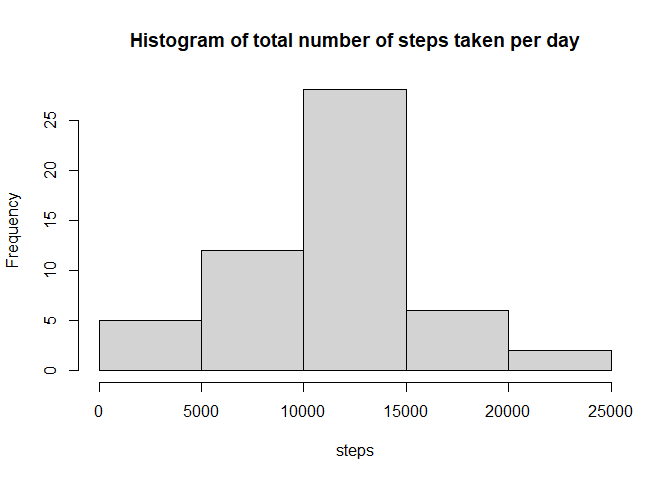
\includegraphics{PA1_template_files/figure-latex/hist_mean_total_daily-1.pdf}

We can also visualize total number of steps taken each day on a graph:

\begin{Shaded}
\begin{Highlighting}[]
\FunctionTok{plot}\NormalTok{(}\AttributeTok{x=}\NormalTok{ tbl}\SpecialCharTok{$}\NormalTok{date, }\AttributeTok{y=}\NormalTok{tbl}\SpecialCharTok{$}\NormalTok{tbl, }\AttributeTok{type=}\StringTok{"l"}\NormalTok{, }\AttributeTok{xlab=}\StringTok{"date"}\NormalTok{, }\AttributeTok{ylab=}\StringTok{"steps"}\NormalTok{, }\AttributeTok{main=}\StringTok{"Total number of steps taken each day"}\NormalTok{)}
\end{Highlighting}
\end{Shaded}

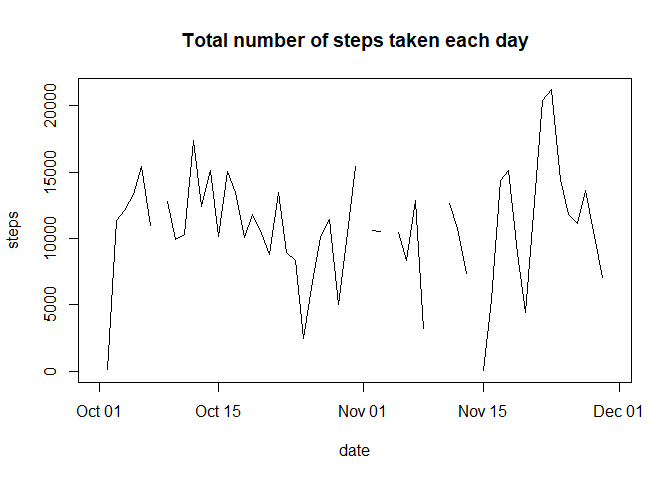
\includegraphics{PA1_template_files/figure-latex/plot_sum_total_daily-1.pdf}

\subsection{What is the average daily activity
pattern?}\label{what-is-the-average-daily-activity-pattern}

Here we can also use \emph{tapply} function to calculate mean of steps
taken within intervals:

\begin{Shaded}
\begin{Highlighting}[]
\NormalTok{tbl }\OtherTok{\textless{}{-}} \FunctionTok{tapply}\NormalTok{(activity}\SpecialCharTok{$}\NormalTok{steps, activity}\SpecialCharTok{$}\NormalTok{interval, mean)}
\NormalTok{tbl }\OtherTok{\textless{}{-}} \FunctionTok{as.data.frame}\NormalTok{(tbl)}
\NormalTok{tbl}\SpecialCharTok{$}\NormalTok{interval }\OtherTok{\textless{}{-}} \FunctionTok{row.names}\NormalTok{(tbl)}

\FunctionTok{plot}\NormalTok{(}\AttributeTok{x=}\NormalTok{ tbl}\SpecialCharTok{$}\NormalTok{interval, }\AttributeTok{y=}\NormalTok{tbl}\SpecialCharTok{$}\NormalTok{tbl, }\AttributeTok{ylim=}\FunctionTok{c}\NormalTok{(}\DecValTok{0}\NormalTok{,}\DecValTok{180}\NormalTok{), }\AttributeTok{type=}\StringTok{"l"}\NormalTok{, }\AttributeTok{xlab=}\StringTok{"intervals during the day"}\NormalTok{, }\AttributeTok{ylab=}\StringTok{"steps"}\NormalTok{, }\AttributeTok{main=}\StringTok{"Average activity pattern throughout the day"}\NormalTok{)}
\end{Highlighting}
\end{Shaded}

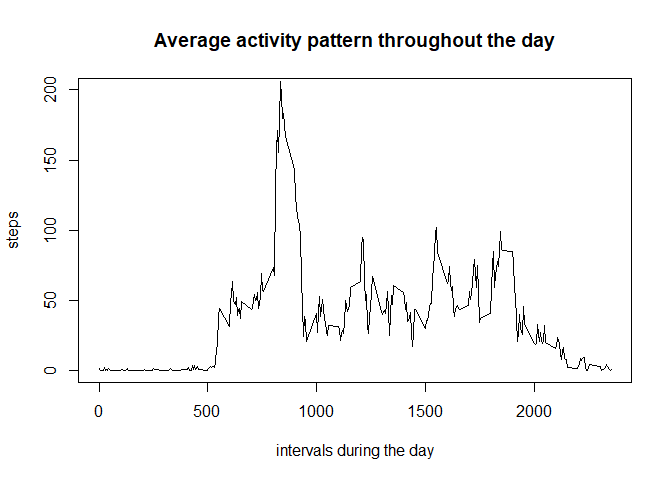
\includegraphics{PA1_template_files/figure-latex/plot_daily_pattern-1.pdf}

The 5-minute interval that, on average, contains the maximum number of
steps:

\begin{Shaded}
\begin{Highlighting}[]
\NormalTok{avgstep }\OtherTok{\textless{}{-}} \FunctionTok{as.data.frame}\NormalTok{(}\FunctionTok{tapply}\NormalTok{(activity}\SpecialCharTok{$}\NormalTok{steps, activity}\SpecialCharTok{$}\NormalTok{interval, mean, }\AttributeTok{na.rm=}\ConstantTok{TRUE}\NormalTok{))}
\FunctionTok{names}\NormalTok{(avgstep) }\OtherTok{=} \FunctionTok{c}\NormalTok{(}\StringTok{"avg\_steps"}\NormalTok{)}
\NormalTok{avgstep}\SpecialCharTok{$}\NormalTok{interval }\OtherTok{\textless{}{-}} \FunctionTok{as.integer}\NormalTok{(}\FunctionTok{row.names}\NormalTok{(avgstep))}
\NormalTok{avgstep[avgstep}\SpecialCharTok{$}\NormalTok{avg\_steps }\SpecialCharTok{==} \FunctionTok{max}\NormalTok{(avgstep}\SpecialCharTok{$}\NormalTok{avg\_steps), ]}
\end{Highlighting}
\end{Shaded}

\begin{verbatim}
##     avg_steps interval
## 835  206.1698      835
\end{verbatim}

\subsection{Imputing missing values}\label{imputing-missing-values}

Let's see how many missing values in the dataset:

\begin{Shaded}
\begin{Highlighting}[]
\FunctionTok{summary}\NormalTok{(activity}\SpecialCharTok{$}\NormalTok{steps)}
\end{Highlighting}
\end{Shaded}

\begin{verbatim}
##    Min. 1st Qu.  Median    Mean 3rd Qu.    Max.    NA's 
##    0.00    0.00    0.00   37.38   12.00  806.00    2304
\end{verbatim}

So there's total of \emph{2304} missing values in the dataset. Total
number of rows in the dataset is: \emph{17568} as we have identified
earlier.

\begin{Shaded}
\begin{Highlighting}[]
\DecValTok{2304}\SpecialCharTok{/}\DecValTok{17568}
\end{Highlighting}
\end{Shaded}

\begin{verbatim}
## [1] 0.1311475
\end{verbatim}

So there's approximately \emph{13\%} missing values.

There's several approaches to imputing the missing values, some of them
are - use mean, median or mode.

Here I will use daily median value for imputing missing values within a
specific day. I will copy \emph{activity} dataset and impute missing
values into copied object.

\begin{Shaded}
\begin{Highlighting}[]
\NormalTok{activity1 }\OtherTok{\textless{}{-}} \FunctionTok{data.frame}\NormalTok{(activity)}
\NormalTok{nas }\OtherTok{\textless{}{-}} \FunctionTok{which}\NormalTok{(}\FunctionTok{is.na}\NormalTok{(activity1}\SpecialCharTok{$}\NormalTok{steps))}

\ControlFlowTok{for}\NormalTok{ (i }\ControlFlowTok{in}\NormalTok{ nas) \{}
\NormalTok{    needed\_date }\OtherTok{\textless{}{-}}\NormalTok{ activity}\SpecialCharTok{$}\NormalTok{date[i]}
\NormalTok{    date\_subset }\OtherTok{\textless{}{-}} \FunctionTok{subset}\NormalTok{(activity, date }\SpecialCharTok{==}\NormalTok{ needed\_date,}
                          \AttributeTok{select=}\FunctionTok{c}\NormalTok{(steps))}
\NormalTok{    median\_day }\OtherTok{\textless{}{-}} \FunctionTok{median}\NormalTok{(date\_subset}\SpecialCharTok{$}\NormalTok{steps, }\AttributeTok{na.rm=}\ConstantTok{TRUE}\NormalTok{)}
\NormalTok{    activity1}\SpecialCharTok{$}\NormalTok{steps[i] }\OtherTok{\textless{}{-}} \ControlFlowTok{if}\NormalTok{(}\FunctionTok{is.na}\NormalTok{(median\_day)) }\DecValTok{0} \ControlFlowTok{else}\NormalTok{ median\_day}
\NormalTok{\}}
\end{Highlighting}
\end{Shaded}

\begin{Shaded}
\begin{Highlighting}[]
\NormalTok{tbl }\OtherTok{\textless{}{-}} \FunctionTok{tapply}\NormalTok{(activity1}\SpecialCharTok{$}\NormalTok{steps, activity1}\SpecialCharTok{$}\NormalTok{date, sum)}
\NormalTok{tbl }\OtherTok{\textless{}{-}} \FunctionTok{as.data.frame}\NormalTok{(tbl)}
\NormalTok{tbl}\SpecialCharTok{$}\NormalTok{date }\OtherTok{\textless{}{-}} \FunctionTok{as.POSIXct}\NormalTok{(}\FunctionTok{row.names}\NormalTok{(tbl))}

\FunctionTok{mean}\NormalTok{(tbl}\SpecialCharTok{$}\NormalTok{tbl, }\AttributeTok{na.rm=}\ConstantTok{TRUE}\NormalTok{)}
\end{Highlighting}
\end{Shaded}

\begin{verbatim}
## [1] 9354.23
\end{verbatim}

So the mean total number of steps taken per day equals \emph{10766.19}.

\subsection{What is median total number of steps taken per
day?}\label{what-is-median-total-number-of-steps-taken-per-day-1}

\begin{Shaded}
\begin{Highlighting}[]
\FunctionTok{median}\NormalTok{(tbl}\SpecialCharTok{$}\NormalTok{tbl, }\AttributeTok{na.rm=}\ConstantTok{TRUE}\NormalTok{)}
\end{Highlighting}
\end{Shaded}

\begin{verbatim}
## [1] 10395
\end{verbatim}

So the median total number of steps taken per day equals \emph{10765}.

Now let's see whether the histogram of the total number of steps taken
each day has changed after missing values were imputed

\begin{Shaded}
\begin{Highlighting}[]
\FunctionTok{hist}\NormalTok{(tbl}\SpecialCharTok{$}\NormalTok{tbl,}\AttributeTok{xlab=}\StringTok{"steps"}\NormalTok{, }\AttributeTok{main=}\StringTok{"Histogram of total number of steps taken per day"}\NormalTok{)}
\end{Highlighting}
\end{Shaded}

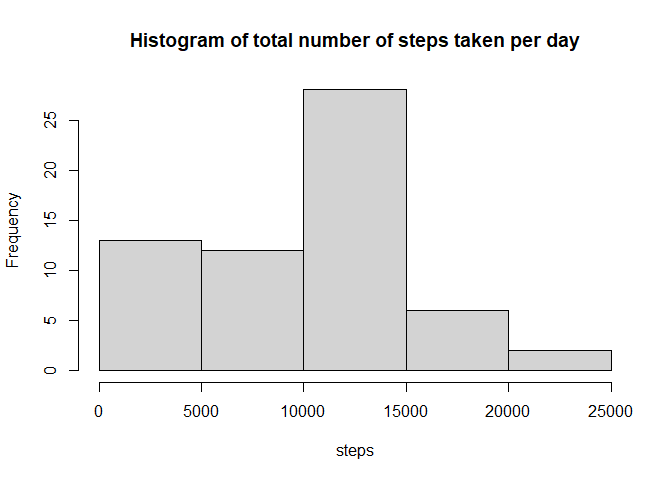
\includegraphics{PA1_template_files/figure-latex/hist_mean_total_daily_after_imputing-1.pdf}

As we can see, the plot did not changed, that's because we used median
for the missing data. For many cases the median is 0, because the
ordered list of step values consists of many zeros.

\subsection{Are there differences in activity patterns between weekdays
and
weekends?}\label{are-there-differences-in-activity-patterns-between-weekdays-and-weekends}

\begin{Shaded}
\begin{Highlighting}[]
\FunctionTok{library}\NormalTok{(ggplot2)}

\NormalTok{activity}\SpecialCharTok{$}\NormalTok{isweekday }\OtherTok{\textless{}{-}} \FunctionTok{as.POSIXlt}\NormalTok{(activity}\SpecialCharTok{$}\NormalTok{date)}\SpecialCharTok{$}\NormalTok{wday }\SpecialCharTok{!=} \DecValTok{6} \SpecialCharTok{\&} \FunctionTok{as.POSIXlt}\NormalTok{(activity}\SpecialCharTok{$}\NormalTok{date)}\SpecialCharTok{$}\NormalTok{wday }\SpecialCharTok{!=} \DecValTok{0}

\NormalTok{weekdays }\OtherTok{\textless{}{-}} \FunctionTok{subset}\NormalTok{(activity, activity}\SpecialCharTok{$}\NormalTok{isweekday }\SpecialCharTok{==} \ConstantTok{TRUE}\NormalTok{)}
\NormalTok{weekends }\OtherTok{\textless{}{-}} \FunctionTok{subset}\NormalTok{(activity, activity}\SpecialCharTok{$}\NormalTok{isweekday }\SpecialCharTok{==} \ConstantTok{FALSE}\NormalTok{)}

\NormalTok{avgstep1 }\OtherTok{\textless{}{-}} \FunctionTok{as.data.frame}\NormalTok{(}\FunctionTok{tapply}\NormalTok{(weekdays}\SpecialCharTok{$}\NormalTok{steps, weekdays}\SpecialCharTok{$}\NormalTok{interval, mean, }\AttributeTok{na.rm=}\ConstantTok{TRUE}\NormalTok{))}
\NormalTok{avgstep2 }\OtherTok{\textless{}{-}} \FunctionTok{as.data.frame}\NormalTok{(}\FunctionTok{tapply}\NormalTok{(weekends}\SpecialCharTok{$}\NormalTok{steps, weekends}\SpecialCharTok{$}\NormalTok{interval, mean, }\AttributeTok{na.rm=}\ConstantTok{TRUE}\NormalTok{))}

\FunctionTok{names}\NormalTok{(avgstep1) }\OtherTok{=} \FunctionTok{c}\NormalTok{(}\StringTok{"avg\_steps"}\NormalTok{)}
\NormalTok{avgstep1}\SpecialCharTok{$}\NormalTok{interval }\OtherTok{\textless{}{-}} \FunctionTok{as.integer}\NormalTok{(}\FunctionTok{row.names}\NormalTok{(avgstep1))}
\NormalTok{avgstep1}\SpecialCharTok{$}\NormalTok{isweekday }\OtherTok{\textless{}{-}} \ConstantTok{TRUE}

\FunctionTok{names}\NormalTok{(avgstep2) }\OtherTok{=} \FunctionTok{c}\NormalTok{(}\StringTok{"avg\_steps"}\NormalTok{)}
\NormalTok{avgstep2}\SpecialCharTok{$}\NormalTok{interval }\OtherTok{\textless{}{-}} \FunctionTok{as.integer}\NormalTok{(}\FunctionTok{row.names}\NormalTok{(avgstep2))}
\NormalTok{avgstep2}\SpecialCharTok{$}\NormalTok{isweekday }\OtherTok{\textless{}{-}} \ConstantTok{FALSE}

\NormalTok{avgstep }\OtherTok{\textless{}{-}} \FunctionTok{rbind}\NormalTok{(avgstep1, avgstep2)}

\FunctionTok{ggplot}\NormalTok{(avgstep , }\FunctionTok{aes}\NormalTok{(}\AttributeTok{x =}\NormalTok{ interval, }\AttributeTok{y =}\NormalTok{ avg\_steps, }\AttributeTok{color =}\NormalTok{ isweekday)) }\SpecialCharTok{+}
   \FunctionTok{geom\_line}\NormalTok{(}\AttributeTok{show.legend =} \ConstantTok{TRUE}\NormalTok{) }\SpecialCharTok{+}
   \FunctionTok{facet\_wrap}\NormalTok{(}\SpecialCharTok{\textasciitilde{}}\NormalTok{isweekday)}
\end{Highlighting}
\end{Shaded}

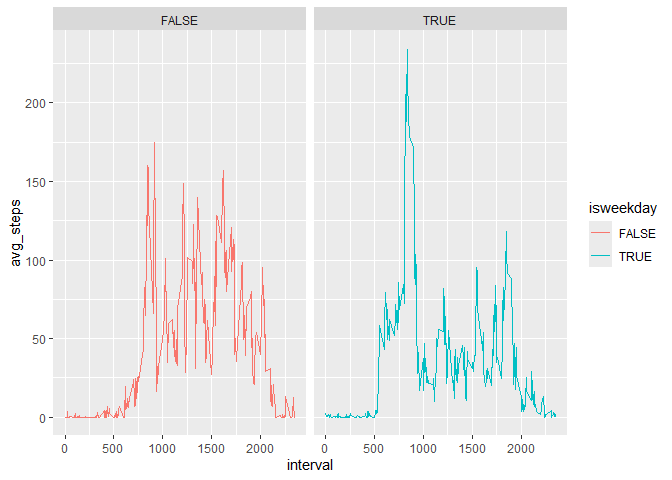
\includegraphics{PA1_template_files/figure-latex/weekdays_weekends-1.pdf}

\end{document}
